%!TEX root = ../main.tex

\chapter{Introduction}
\label{ch:intro}
% \vspace{2em}
\section{Blockchain Overview}
Blockchains shake the industry, academia, and the entire world with storms. 
The swing of the butterfly that initiates the storm is an unidentified hacker named Satoshi Nakamoto, who authored the Bitcoin whitepaper in 2008~\cite{nakamoto2019bitcoin}. 
His proposal makes the breakthrough by employing Proof-of-work (PoW) mechanism, which allows mutually distrusting parties to reach an agreement on the ledger.
The ledger records the forever-appending monetary transactions, with the immutability guarantee. 
Along with other cryptographic techniques, such as the asymmetric encryption, the Merkle index, and the hashed chain structure, Bitcoin is the first-ever practical cryptocurrency that operates under a pure peer-to-peer network, without any central authority. And it immediately follows a series of alt-coins variants~\cite{wiki:List_of_cryptocurrencies}. 
Bitcoin is ground-breaking, as no early design can reach such scalable Byzantine consensus while defying Sybil Attacks. 
Nakamoto overcomes it by relying on the built-in cryptocurrency to regulate the participant behavior via the economic incentive. 

To further unleash the power of blockchains beyond the cryptocurrency, there are two distinct directions. 
On the one hand, researchers preserve the incentive-based consensus to resolve the anonymity in the open setting. 
But it extends the system functionality from simple monetary flow into arbitrary data transformation, powered by smart contracts. 
A typical example is Ethereum, which allows to encode Turing-complete logic and execute it on an embedded virtual machine. 
We refer to this class of blockchains, featured with incentive-based consensus, built-in cryptocurrencies and the unauthenticated setup as \textit{permissionless blockchains}. 

On the other hand, to cater for applications where authenticity and auditability are already mandated, blockchain designers take advantage of their close membership, and turn for more efficient and established state-machine replication~\cite{schneider1990implementing} for the consensus. 
In addition, without the built-in cryptocurrencies, the smart contracts of these blockchains are more oriented towards their specific domains, such as Corda~\cite{hearn2016corda} for the financial sector and Hyperledger Fabric~\cite{androulaki2018hyperledger} for the enterprise. 
We refer to the above class of blockchains \textit{permissioned}.
Permissioned blockchains shows more potential to disrupt the industry and attract more interest from entrepreneurs. 

Despite the above differences, both classes of blockchains share the identical high-level architecture, as proposed in BLOCKBENCH~\cite{dinh2017blockbench} and illustrated in Figure~\ref{fig:intro:arch}. 
The architecture is layered into four. Enumerating from the top, they are the application, consensus, execution, and data model layer. 
A typical processing pipeline for a generic blockchain constitutes of the following procedures. 
The consensus layer continuously drives participants to reach an agreement on the block at the ledger tip. 
Each participant then invoke the contract to mutate the state, based on the context in each transaction in the block. 
This step is conducted at the execution layer.
If a transaction conforms to the blockchain protocol, the participant then persists its effect in the data model layer. 
And the top application layer hides all the underneath processing details but leaves interfaces to accept the request and query the ledger. 

\begin{figure}[!t]
  \centering
  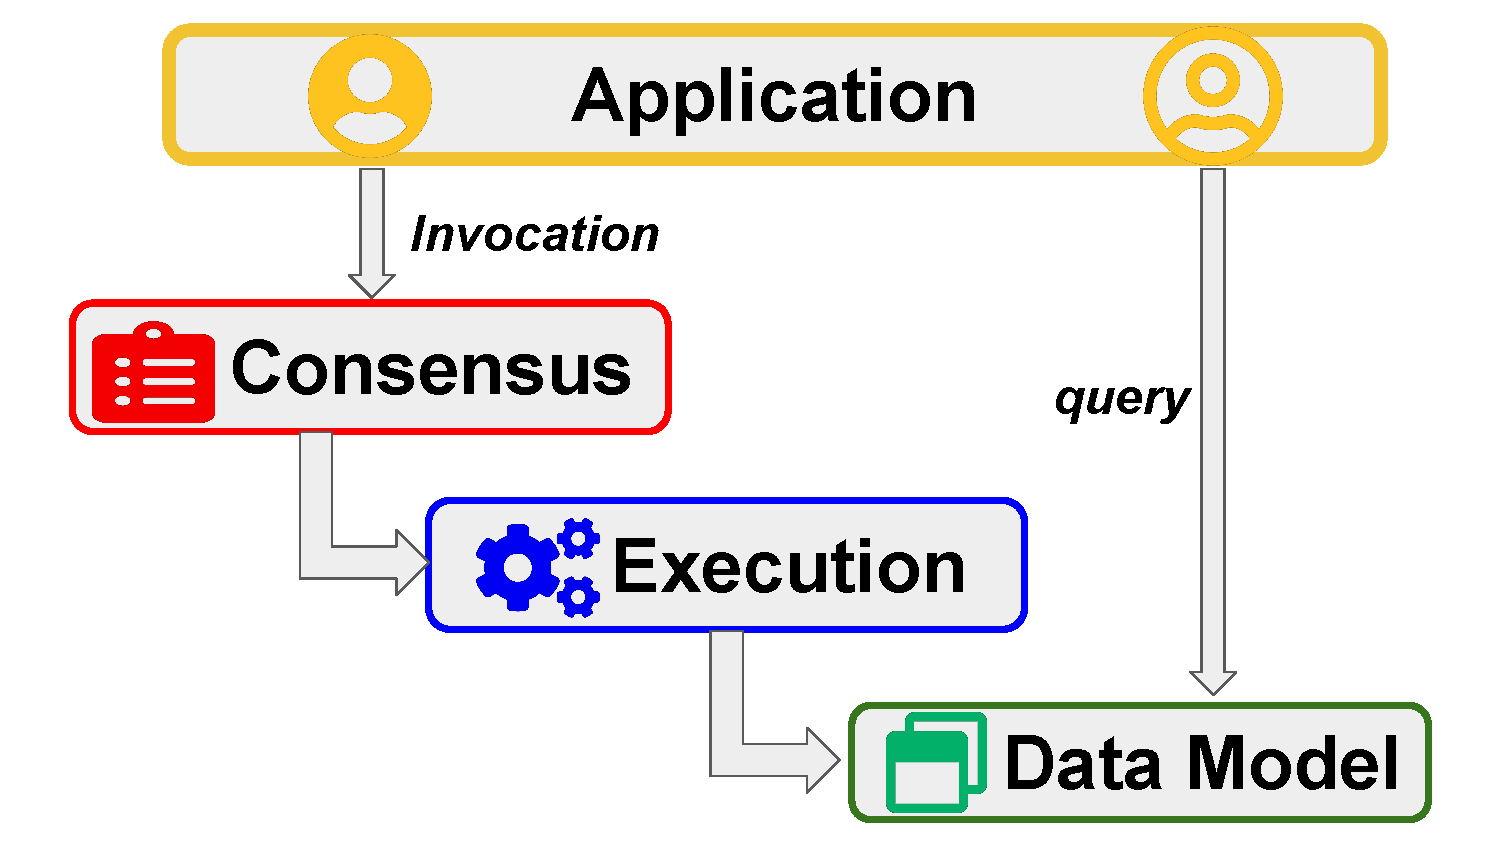
\includegraphics[width=0.8\linewidth]{diagram/intro/architecture.pdf}
  \vspace{\BeforeCaptionVSpace}
  \caption{Blockchain high-level architecture. }
  \subcaption*{State-mutating transactions must undergo the consensus and the execution components before persisting their effects at the data model layer, whereas ledger and state queries are directly answered by the storage component. }
  \label{diagram:intro:arch}
\end{figure}

\section{Vision, Motivation and Principle}

Our system-wide optimization primarily focuses on permissioned blockchains.
When compared with permissionless blockchains, permissioned blockchains resembles more to distributed databases and hence are more applicable to the database techniques.  
Their similarities and implication are summarized as follows: 

\textbf{Generic Workload Support. } 
Smart contracts of permissioned blockchains support arbitrary data transformation, like stored procedures in databases. And both of their invocation result into a transaction in their respective context. 
This is in contrast with permissionless blockchains, which mostly restrict their attention to the ownership transfer. 
Inevitably, permissioned blockchains raises for more challenges due to their generality.
Our optimization can no longer exploit the strong notion of asset ownership like in permissionless blockchains. 

\textbf{Authenticated Identity. } 
Analogous to distributed databases, permissioned blockchains operate under the authenticated setup.
Hence both categories of systems allow for more efficient state-machine replication consensus to withstand the byzantine failure. 
In comparison to permissionless blockchains, their PoW-like consensus (which is a must to mitigate Sybil Attacks) dominates the entire system performance. 
From this angle, the enhancement on other components of permissioned blockchains is necessary and worthwhile, as to side with their faster state-machine replication approach. 
Furthermore, the known membership relieves us from the identity problem. 
So that we will never get plagued by any Denial-of-the-service Attacks or Sybil Attacks throughout. 

The above commonalities explain why a number of entrepreneurs are actively exploring permissioned blockchains to replace their enterprise-ready databases. 
They seek to harness their common data processing capability while enjoying the additional decentralization and security that permissioned blockchains uniquely provide. 
However, their attempts are primarily hindered by the following limitations of the permissioned blockchains:

\textbf{Utility. }
Even though smart contracts open us opportunities for arbitrary transaction logic for blockchains, their provided utility is far from comparable to that of databases. 
For example, mainstream blockchains only provide procedural languages to encode the data transformation, such as Ethereum with Solidity and Hyperledger Fabric with Golang. 
But current relational databases already adopt the more expressive declarative SQL language, not to mention the enriched query features that databases develop over decades. 
In the face of growing demand, permissioned blockchains call for more data processing functionalities, like databases. 

\textbf{Performance. }
Another challenge is the low processing volume of permissioned blockchain to accommodate the business load. 
Researchers in BLOCKBENCH evaluated three blockchains with database workloads on the same testbed. 
Their results show that blockchains lag far behind databases in around two magnitudes. 
We believe the extra security properties of blockchains shall not solely account for such a huge performance gap. 
There must exist abundant optimization room available for the speedup. 

In the above, we lay out the optimization vision by showing vast similarities between permissioned blockchain and distributed databases. 
And we have also motivated such necessity by pinpointing the pain points for the adoption of blockchains in the industry. 
We now explain the three principles that our enhancement follows:

\begin{itemize}
  \item We break no security properties. We believe security lies at the core of blockchains. Although relaxing security assumptions is a standard engineering approach for the performance speedup, we do not find it scientific. A typical approach is to improve the system throughput by simply switching from byzantine tolerant consensus to crash failure tolerant. In our thesis, this principle can be manifested in the following two ways. Firstly, for the utility enhancement, we must preserve security on the added features. For instance, in Chapter~\ref{ch:prov}, we take special care to extend the tamper-evidence guarantee to the data provenance. On the other hand, any proposed procedures must be accompanied by their security analysis. This is why we dedicate a subsection in Chapter~\ref{ch:txn} on the security implication of the transaction reordering. 
  \item We adopt the modularized approach. We decouple a complex system into individual layers for the separate optimization. Modularization allows for the separation of concerns for the ease of reasoning. It also facilitates interoperability with independent optimization. 
  We follow the proposed architecture in BLOCKBENCH for our blockchain optimization in Chapter~\ref{ch:prov} and ~\ref{ch:txn}. In particular, we pinpoint our instrumentation with respect to each of four layers, as classified in Figure~\ref{diagram:intro:arch}. 
  \item Rather than building from the scratch, we ground our optimizations on Hyperledger Fabric v2.2, the most popular permissioned blockchain, for the demonstration. Building on an existing system not only reuses its well-examined components, but this action by itself proves our practicality. Moreover, the results from a full-fledged system, instead of a prototype, are more convincing. And the evaluation is more meaningful when directly comparing with the vanilla baseline. 
\end{itemize}

\section{Optimization Basis}
We incrementally apply our optimization on Hyperledger Fabric 2.2.0 into {\fs} and open source it~\cite{fsharp}. We fork its codebase with the commit hash \textit{2821cf}, the last commit on the branch \textit{release-2.2} when we start preparing this thesis. In later paragraphs, Fabric, without any version specification, all refers to this codebase snapshot. 

We now evaluate its throughput under its off-the-shelf configuration, which serves as the baseline. 
Unless otherwise mentioned, all our following experiments in this thesis are conducted in the same testbed as this experiment.
The testbed consists of a local cluster of 16 nodes. Each node is equipped with E5-1650 3.5GHz CPU, 32GB RAM, and 2TB hard disk. The nodes are interconnected via 1Gbps Ethernet. 

We present the primary results, after averaging over 3 times on the four-peer setup, in Figure~\ref{chart:intro:basic}. 
The first workload consists of no-op transactions that access no records. 
Fabric keeps around only 2300 tps throughput when the number of transactions per block is 2000 and beyond. 
In the second workload with 2000 transactions per block, we gradually increase the request skewness in the modification workload, in which each transaction reads and updates a single record out of 10k. 
The request distribution follows Zipfian distribution, where the larger coefficient $\theta$ implies for more skewness. 
When $\theta$ reaches 1.0, we observe its throughput reduces to 549 tps, 65\% of that when $\theta=0$. 
And more than half of transactions in the ledger do not take effect due to the transactional conflicts. 
This primary experiment further motivates for the performance speedup of permissioned blockchains. 

\begin{figure}[tp]
	\centering
    \begin{subfigure}{0.45\textwidth}
      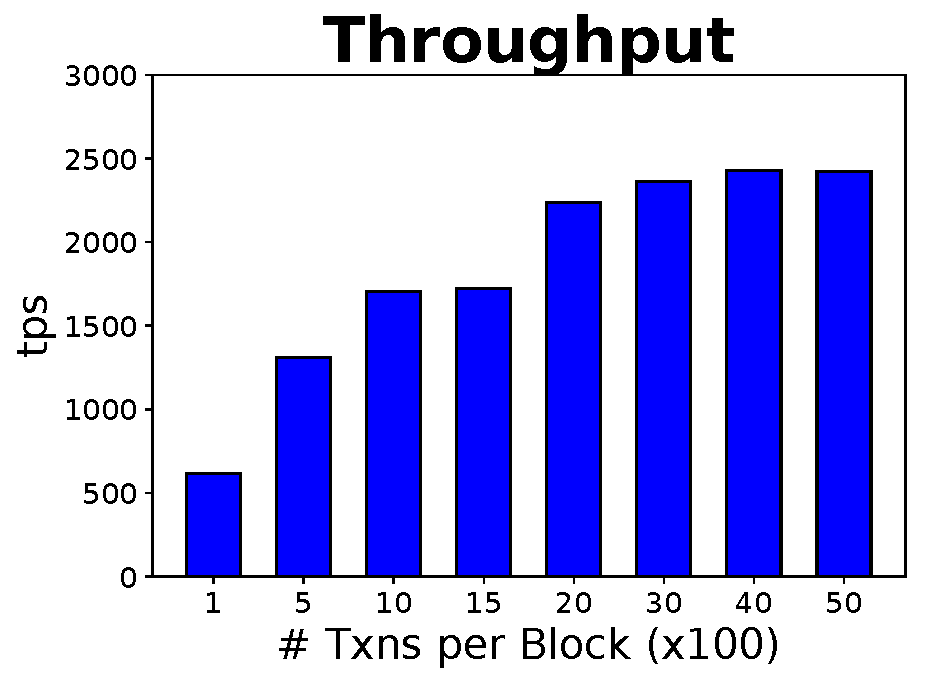
\includegraphics[width=0.99\textwidth]{chart/intro/noop.pdf}
    \end{subfigure}
    \begin{subfigure}{0.45\textwidth}
      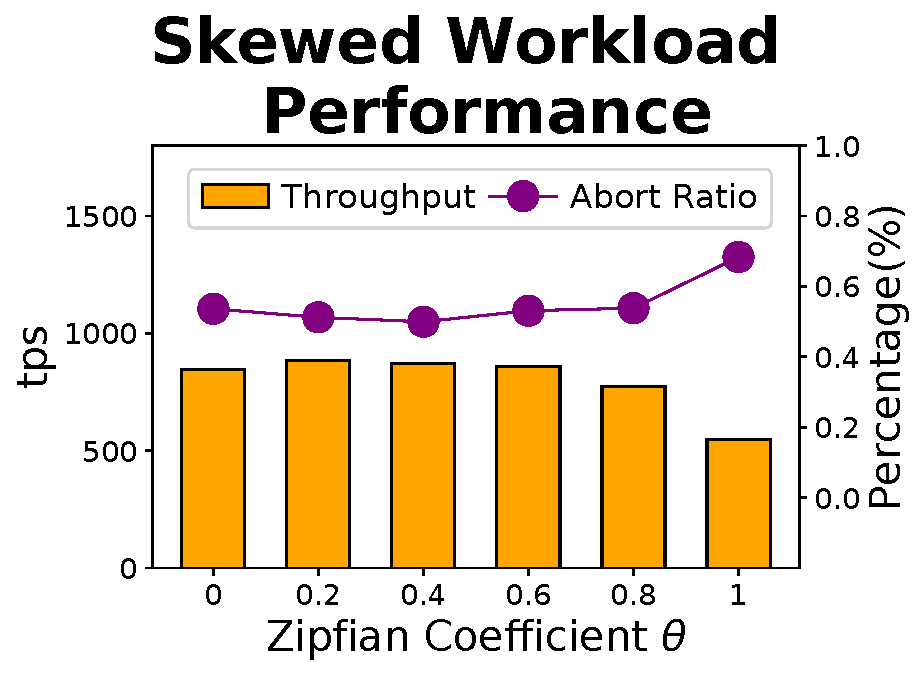
\includegraphics[width=0.99\textwidth]{chart/intro/skew.pdf}
    \end{subfigure}
    \caption{Primary evaluation results for Fabric. }
    \label{chart:intro:basic}
    % \vspace{-1.0em}
\end{figure}

\section{Thesis Synopsis}
We structure the rest of this thesis as follows. Chapter~\cite{ch:literature} overviews the recent year progress on both permissioned and permissionless blockchains. The covered literature spans from the database, distributed computing, and security communities. For the modularized fashion, we organize their reviews according to the classified layers in Figure~\ref{diagram:intro:arch}. This chapter ends with our critical analysis in this area. 

Chapter~\ref{ch:twin} proposes a taxonomy that unifies blockchains and distributed databases. 
The study considers both systems as the same type of distributed transactional systems, for the joint analysis on their respective focus. 
According to each dimension in the taxonomy, we devise corresponding workloads for the evaluation. 
Our results reveal the implication of their design choices. 
This comprehensive study sheds light on the optimization opportunities on permissioned blockchain with database techniques. 

Chapter~\ref{ch:prov} demonstrates our optimization for the utility. 
We first explain the added business value when data provenance is exposed to smart contracts. 
Then we introduce how lineage information in blockchains are captured, stored, and queried. 
The greatest contribution of our proposal is to extend the integrity property for the entire data evolution history. 
After implementing it into {\fs}, the empirical evaluation demonstrates the negligible performance and storage overhead with this additional feature. 

Chapter~\ref{ch:txn} demonstrates another optimization on the performance. 
The work originates from our following subtle observation:
the execute-order-validate architecture in permissioned blockchains may over-abort transactions under the Serializable isolation level. 
Borrowed from the well-established transactional analysis from databases, we reason about the potential of transaction reordering to streamline the execution schedule. Based on the developed insight, then we adapt {\fs} to attain the theoretical limits. 
And the improvement is empirically demonstrated with the remarkable speedup, compared with the vanilla Fabric and the state-of-the-art. 

At last, we wrap up the thesis with the conclusion and future directions in Chapter~\ref{ch:conclu}. 

